\documentclass[11pt]{article}

\usepackage{fancyhdr}
\usepackage{natbib}
\usepackage{amsmath}
\usepackage{swmacros}
\usepackage{graphicx}
\usepackage{float}
%\usepackage[top=1in, bottom=1in, left=.5in, right=.5in]{geometry}
%\usepackage[font=small,labelfont=bf]{caption}

\setlength\parindent{0pt}
% Title.
% ------
\title{STAT 240 Final Project}
\author{Rebecca Barter, Andrew Do and Kellie Ottoboni}



\begin{document}

\maketitle

 \section{Introduction}
Over the last two decades developing countries have seen an increase in the number of new primary school entrants, driven in part, by the elimination of school fees. For example, between 1999 and 2004 the number of new entrants to primary school in sub-Saharan Africa increased by more than 30 percent (\cite{unesco2007}). Although this influx of new students is undeniably a positive development, steps needs to be taken to ensure that the quality of education is not diminished. For example, by 2005, the average first grade class size in Kenya had swelled to 83, with 28 percent of first grade classes containing more than 100 students (\cite{duflo2007}). Moreover, many of the new students were significantly less prepared than those in the past.\\
Unfortunately, little prior work had been undertaken to evaluate the most effective methods of handling such an influx of students. In a randomized experiment, Duflo et al. aim to answer several questions related to a number methods of resource allocation in primary education. In particualr, the investigators aim to assess the impact of reduction in pupil-teacher ratios, implementing tracking (separating classes into high and low streams based on prior test scores) and different institutional environments (type of teacher, and whether or not the school undertakes teacher monitoring and education).\\
 In this report, we investigate the data obtained from the study undertaken by Duflo et al, with a focus on evaluating the impact of tracking on student achievement. 
 
 \section{Tracking}
Tracking involves separating pupils by academic ability within schools. In particular, a student is assigned to the high stream if their prior achievement is above the median, and is assigned to the low stream otherwise. There have been multitudes of studies involving the effects tracking in developed countries, with no overall consensus on whether it is beneficial or detrimental to future student achievement. However those who claim that tracking is beneficial to students have several arguments. For example the reduced skill differential has the potential to allow for better lesson execution and time allocation by teachers; they can focus on teaching at a level that will benefit all students in the class, rather than having to cater to a wide range of abilities. Further, it is possible that ensuring that students are placed in classes of the appropriate difficulty levels will reduce behavioral outlashing by students. Finally, proponents argue that the ``value-added'' is maximized within each group.\\
In contrast, critics of tracking argue that in the absence of tracking, high performing students are given the opportunity to practice synthesis by teaching low performers. Further, they pose the idea that tracking is a self-fulfilling prophecy; students in the low stream will achieve lower than they otherwise might, simply because they have been put in a class that implies that they are not as able. This idea is reinforced by the argument that teachers may require less of students in the low stream, and thus that the education gap will widen between the high and low achieving groups.\\
Through our analysis of the data provided by Duflo et al., we will provide data-driven evidence for several of these arguments, and present our position on the effects of tracking on disadvantaged schools in Kenya. In particular, we aim to answer whether 1) there is value-added by introducing tracking, 2) whether tracking has a differential effect on different strata of students, and 3) whether tracking creates a gap between students of approximately average ability, since these students can be considered to be randomly assigned to the low and high streams.
 
 \section{Study Design}
 
 The study conducted by Duflo et al. involves data from a randomized experiment spanning 18 months involving the first grade class from 210 primary schools in Western Kenya. These schools have a combined 21,000 students and prior to the experiment each school has only a single first grade class taught by a centrally-hired teacher with civil service protection (hereafter referred to as a ``civil service teacher''). The study involves several layers of randomization which are summarized in Figure~\ref{fig:randomization}. The ``Extra Teacher Program'' (ETP) provided funds to 140 schools randomly selected from the pool of 210 schools to hire an extra teacher for first grade classes. These teachers were hired locally, and earned approximately a quarter of the civil service teachers, but had the same academic qualifications. In 70 of these 140 ETP schools tracking was introduced (these schools are ``tracked'' schools), whereby the two classes were divided by initial achievement, and the classes were randomly assigned to either a civil service teacher or a contract teacher. In the other half of the ETP schools (``non tracked'' schools), students were randomly assigned to either the local contract teacher or the existing civil service teacher. Finally, half of the 70 non-tracked ETP schools and half of the tracked ETP schools were given funds to empower the local school committee to monitor and train teachers (these schools are referred to as the ``monitored'' schools).
 
 \begin{figure}[H]
 \centering
 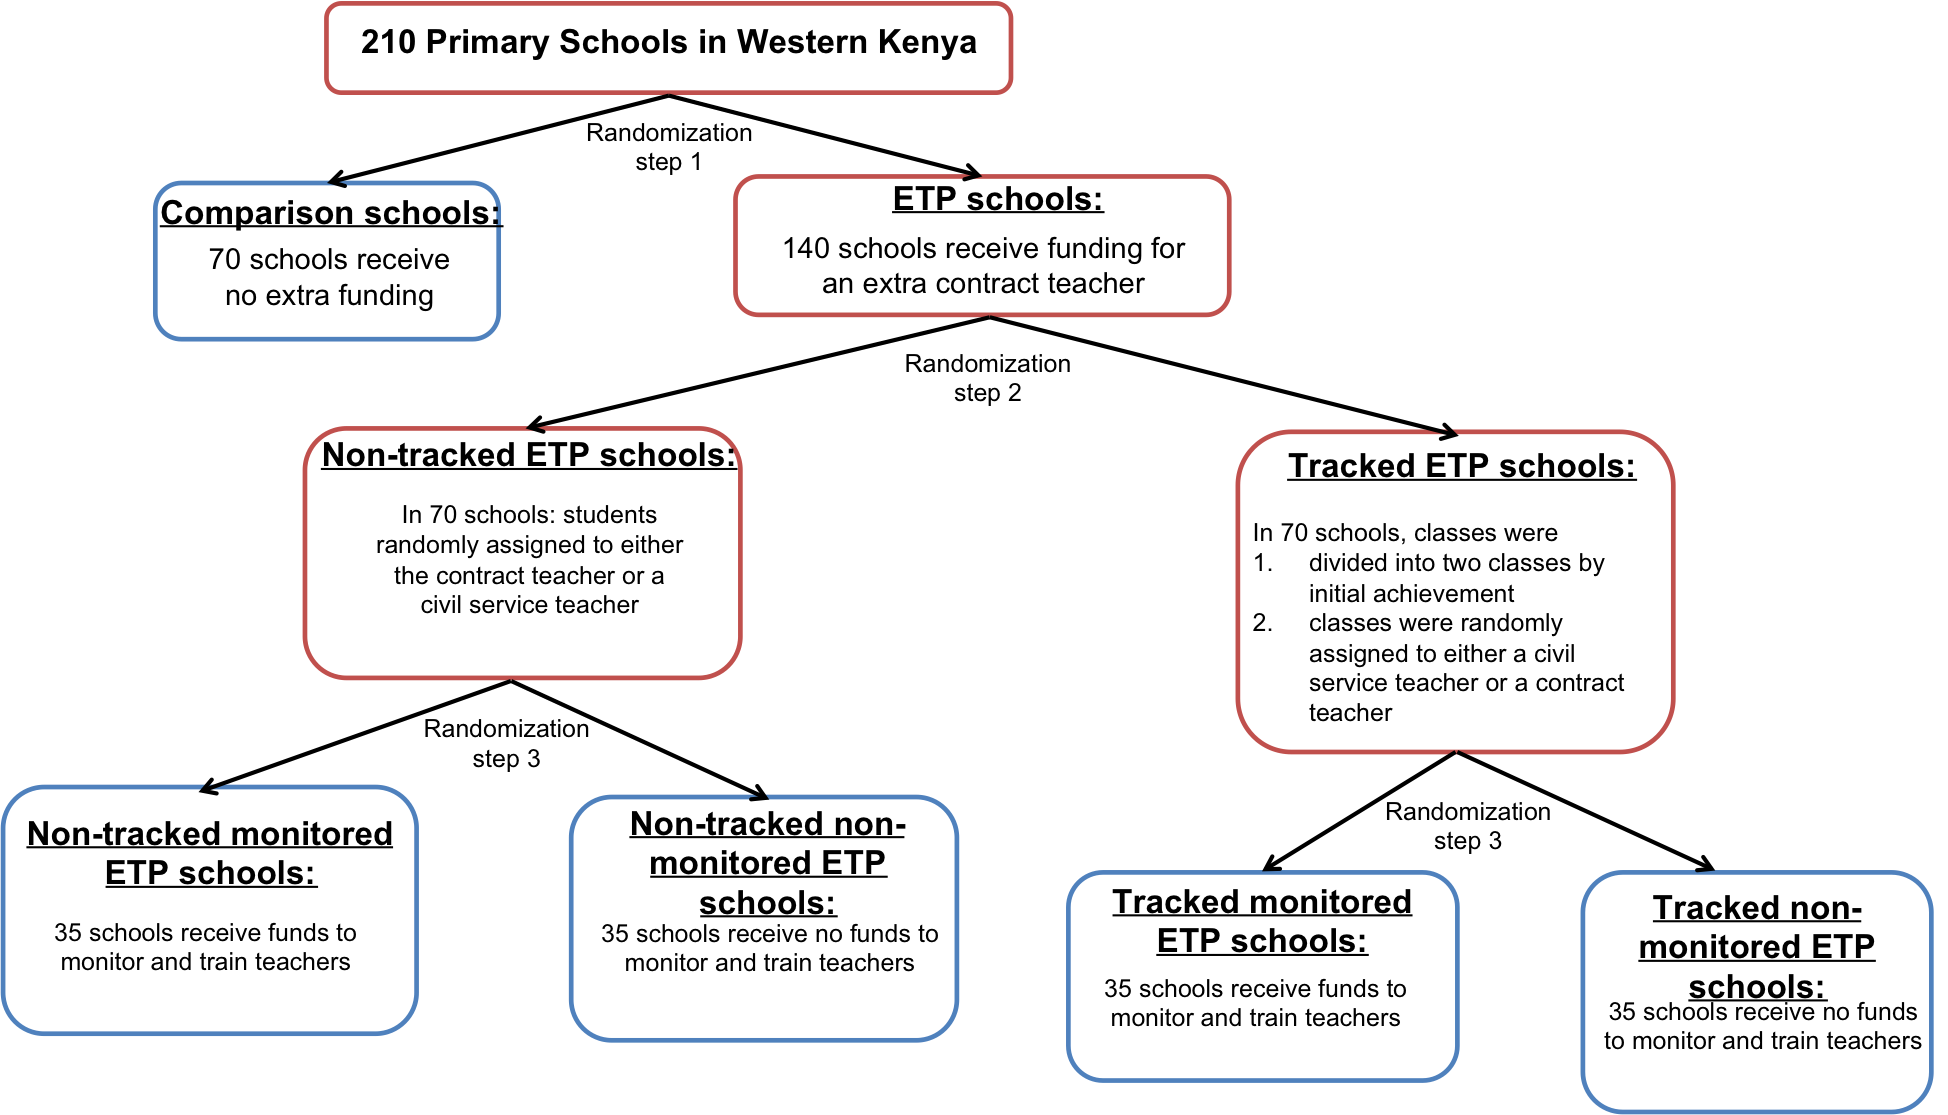
\includegraphics[scale=0.5]{Randomization_flow.png}
 \caption{A flowchart describing the randomization steps of the study}
 \label{fig:randomization}
 \end{figure}
 
Stream assignment in tracked schools was based on initial test scores (baseline test) which were administered locally within schools. Thus these baseline test scores are internally consistent within schools but not comparable across schools. The success of the program was assessed based on scores from a standardized mathematics and language test taken by 60 students from each school (approximately 7000 students all together) after 18 months (the end line test). Another test was also taken by the same students after 24 months (the long-term followup test). We note that the ETP funding ceased after the 18 month endline, so the tracking was no longer in place at the 24 month followup. These tests contained numeracy and literacy questions ranging from counting and identifying letters to subtracting two-digit numbers and writing words.
 
 \section{Exploratory Data Analysis}
 
 \section{Analysis}
 \subsection{Value-added over time by tracking}
Unfortunately since the baseline test scores were not comparable across different schools, we were unable to measure the value-added from tracking by comparing baseline with the 18 month endline scores. As a result, we thus chose to measure the long-term value-added by comparing 18 month endline scores with the 24 month follow-up scores. This comparison allows us to see if tracking yielded a lasting effect on students, even after the tracking was no longer in place.

 \subsection{Stratified permutation tests for comparing tracking with non tracking schools}
In comparison to the previous analysis, which involved comparing scores over time for the students in tracking schools, we now turn to a comparison of scores achieved by students in tracking schools with students in non-tracking schools.
 
 \subsection{Regression discontinuity for comparing students in the high stream with those in the low stream}
We now aim to analyze the effect of stream assignment on students in tracked schools who initially achieved near the cutoff point. This analysis is based on the idea that students who achieved near the cutoff point have approximately equivalent abilities and it was random noise that lead to their assignment into either the high or low stream. For example, if a student slept poorly the night before the baseline test, they may have scored a few points below the cutoff point, whereas they may otherwise have scored a few points above the cutoff point. As a result, we can consider the students whose initial scores fall within a small window of the cutoff point as being randomly assigned into either the high or low stream.
 
 
 
 \section{Conclusion}
 
 
 \bibliographystyle{apalike}
\bibliography{references}
 
\end{document}
